
\section{Integrated circuits structure \ddcnew}
For the purpose of properly introducing the electrical models I developed for \bbi, it is required, in the first place, to have a look at how integrated circuits are structured.
It involves analyzing the different structures composing an IC, such as:
\begin{itemize}
    \setlength\itemsep{-0.1em}
    \item Its power supply plan, consisting in various metal levels stacked one on top of the others;
    \item The standard-cells: pre-characterized cells used as elementary building blocks;
    \item The various substrate types, such as dual-well and triple-well not to cite them all.
\end{itemize}

    \subsection{Power supply rails \ddcnew}
    \begin{figure}[ht]
    \centering
    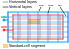
\includegraphics[width=0.45\textwidth]{3_modeling/figures/IC_POWER_PLANS.pdf}
    \caption{Coarse traditional IC power delivery diagram, showing a standard-cell segment sandwiched between power rails.}
    \label{fig:icPowerRail}
\end{figure}
    In most modern integrated circuits, power is brought to the transistors through various metal layers organized as meshes.
    The resulting meshes bring the power to the transistors, aka the logic gates, aka the Standard-Cells.
    There are one or more pads for each power signal (typically called VDD and GND), connecting to power rings, surrounding the IC silicon die, as shown in Fig. \ref{fig:icPowerRail}.
    Then, power straps are created to mesh the rings and distribute evenly the power to the transistors.
    After that, rails are drawn to connect the power to the standard-cell segments, and vias are placed between rails and straps to wire them together.

    \subsection{Standard-Cell rows \ddcnew}
    \begin{figure}[ht]
    \centering
    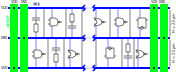
\includegraphics[width=0.55\textwidth]{3_modeling/figures/std_cell_segment_principle.pdf}
    \caption{Symbolic view of a Standard Cell Segment, surrounded by its local power delivery network.}
    \label{fig:istdCellRows}
\end{figure}
    As I have said previously, Standard-Cells are the elementary building blocks used to design ICs.
    They are pre-defined logic cells, fulfilling a specific logic function.
    Standard-Cells can then be connected together to form a complete logic function.
    They are usually organized in rows, with a fixed height and variable width depending on the function.
    This allows simple power connection to each Standard-Cell.
    Fig. \ref{fig:istdCellRows} illustrates how Standard-Cells are routed in an IC design.
    At the top of the Standard-Cells is the VDD power input, and at the bottom the GND power input.
    Typically, without considering various technologies, between the power rails are trapped three main regions:
    \begin{itemize}
        \setlength\itemsep{-0.1em}
        \item A N-doped silicon area, called the N-well, where the PMOS transistors are lithographed;
        \item A metal area where the transistor gates are accessible;
        \item A P-doped silicon area, called the P-well, where the NMOS transistors are lithographed.
    \end{itemize}
    Therefore, NMOS transistors are located in the bottom half of the standard-cell, and the PMOS are located in the top half.

    \subsection{Various substrate types \ddcnew}
    \begin{figure}[htbp!]
    \centering
    %\scriptsize
    % \setstretch{0.9}
    \begin{subfigure}{7.8cm}
        % \def\svgwidth{9.0cm}
        \includegraphics[width=7.8cm]{3_modeling/figures/DUAL.pdf}
        \caption{Dual-Well}
        \label{subfig:dualIvx}
    \end{subfigure}
    \begin{subfigure}{7.8cm}
        % \def\svgwidth{9.0cm}
        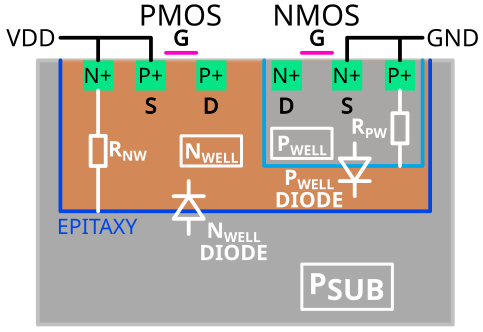
\includegraphics[width=7.8cm]{3_modeling/figures/TRIPLE.pdf}
        \caption{Triple-Well}
        \label{subfig:tripleIvx}
    \end{subfigure}
    \caption{Dual-well and triple-well inverter silicon sectional view.}
    \label{fig:dualTripleIvx}
\end{figure}
    Because there are various ways to lithograph transistors for a given technology, I decided to linger and analyze the differences of two substrate types commonly found in bulk technologies:
    \begin{itemize}
        \setlength\itemsep{-0.1em}
        \item Dual-well substrates, where NMOS transistors are lithographed directly into the P-doped silicon substrate;
        \item Triple-well substrates, where the NMOS transistors are lithographed into a buried P-well inside the N-well where the PMOS are lithographed.
    \end{itemize}
    For the purpose of illustrating the structural differences between those substrate types, I am going to use the schematics displayed in Fig. \ref{fig:dualTripleIvx} as a guide, illustrating the cross-sectional view of a logic inverter created in both a dual-well and a triple-well substrate.

        \subsubsection{Dual-well substrates \ddcnew}
        To begin with, let us focus on dual-well substrates.
        A schematic sectional view of a CMOS inverter manufactured in a dual-well substrate is shown in Fig. \ref{subfig:dualIvx}
        Among moderately old ICs, it was common to find dual-well substrates.
        In these substrates, NMOS transistors are lithographed directly into the P-doped silicon substrate, as we can see in Fig. \ref{subfig:dualIvx}.
        In addition to this, a N-doped silicon area is created inside the P-substrate, called the N-well, to lithograph the PMOS transistors.
        This results in a silicon junction, electrically represented by the N-well diode on the schematic, and called the epitaxy, highlighted in saturated blue.
        Because doped silicon does have a non-zero resistivity, electrical resistances are represented to demonstrate this:
        \begin{itemize}
            \setlength\itemsep{-0.1em}
            \item $RC_{VDD}$ represents the access resistance measured between the epitaxy and the PMOS transistor through the N-well;
            \item $RC_{GND}$ is the access resistance measured between the epitaxy and the NMOS transistor through the P-substrate.
        \end{itemize}

        \subsubsection{Triple-well substrates \ddcnew}
        \textcolor{orange}{TW helps to reduce crosstalk noise.}
        On the other hand, triple-well substrates are also commonly used, often in combination with dual-well on the same die, to provide an electrical isolation between NMOS and PMOS transistors.
        It is achieved by creating inside the N-well, another doped silicon area, inversely doped, called the P-well.
        Inside the latter are then lithographed the NMOS transistors, while the PMOS transistors are still lithographed inside the N-well.

\section{Standard-Cell Segment (SCS) and their models \ddcnew}
Thanks to what I have introduced in the previous section, that is, the Standard-Cell arrangement used to create IC architectures, alongside the two identified substrate types of interest: Dual-Well and Triple-Well, it is now possible to elaborate an electrical model for such integrated circuits.
Because I am differentiating \dwF and \twF substrates, I am introducing two separate models, even though they show some similarities.

The models I developed are an improvement over the electrical models proposed by M. Dumont for \emfi \cite{mathieuEMFI}.
Similar to \cite{mathieuEMFI} and to VLSI design, I am using the Standard-Cells as a basic building block.
However, in my model is not represented the logic function of a Standard-Cell, rather its electrical behavior.
More specifically, the elementary building block of the proposed electrical model represents the average electrical behavior of several Standard-Cells, called Standard-Cell Segment (\scs).

\begin{figure}[ht]
    \centering
    \includegraphics[width=0.65\textwidth]{3_modeling/figures/substrateSubdivision_6.pdf}
    \caption{Substrate subdivision improvement over M. Dumont model for \emfi \cite{mathieuEMFI}. The backside is the accessible substrate, and the epitaxy is the highest substrate level, a.k.a. the silicon junction between the P-substrate and the N-well.}
    \label{fig:surfaceSubDivid}
\end{figure}
Because I based my work on M. Dumont model \cite{mathieuEMFI}, I have made modifications to it.
The major modification is displayed in Fig. \ref{fig:surfaceSubDivid}.
In M. Dumont model, the silicon P-substrate is represented solely thanks to a network of 6 resistors.
However, when performing \bbi, the substrate is the main physical environment where the electric charges travel.
Therefore, as I describe in more details further, it is required to improve the spatial resolution of the model, as shown in Fig. \ref{fig:surfaceSubDivid}.
This is done by splitting the substrate electric model in several 6-resistors networks interconnected with each other, thus aloowing for more precise analysis of the substrate charges.

\begin{figure}[ht]
    \centering
    %\scriptsize
    % \setstretch{0.9}
    \begin{subfigure}{0.45\textwidth}
        % \def\svgwidth{9.0cm}
        \includegraphics[width=\textwidth]{3_modeling/figures/dualWell_no_5e.pdf}
        \caption{Dual-Well}
        \label{subfig:dualScs}
    \end{subfigure}
    \hfill
    \begin{subfigure}{0.45\textwidth}
        % \def\svgwidth{9.0cm}
        \includegraphics[width=\textwidth]{3_modeling/figures/tripleWell_no_5e.pdf}
        \caption{Triple-Well}
        \label{subfig:tripleScs}
    \end{subfigure}
    \caption{Three-dimensional Dual-Well and Triple-Well IC comprehensive standard-cell electrical schematic.}
    \label{fig:dualTripleScs}
\end{figure}
Fig. \ref{fig:dualTripleScs} shows the 3-dimensional view of the developed models for my thesis.
The next subsections are dedicated to describing these models both for \dwF and \twF substrates.

    \subsection{The case of Dual-Well substrates \ddcnew}
    Fig. \ref{subfig:dualScs} shows the electrical model of an SCS for \dwF substrates.
    Each SCS is delimited by the P-substrate at its bottom (\ovalbox{1}) and by the power rails at its top (\ovalbox{5}, \ovalbox{5'}).

    \subsection{The case of Triple-Well substrates \ddcnew}

\section{Electrical models \ddcold}
\label{sect:elecModels}
%\begin{figure}[htbp!]
    \centering
    %\scriptsize
    % \setstretch{0.9}
    \begin{subfigure}{7.8cm}
        % \def\svgwidth{9.0cm}
        \includegraphics[width=7.8cm]{3_modeling/figures/DUAL.pdf}
        \caption{Dual-Well}
        \label{subfig:dualIvx}
    \end{subfigure}
    \begin{subfigure}{7.8cm}
        % \def\svgwidth{9.0cm}
        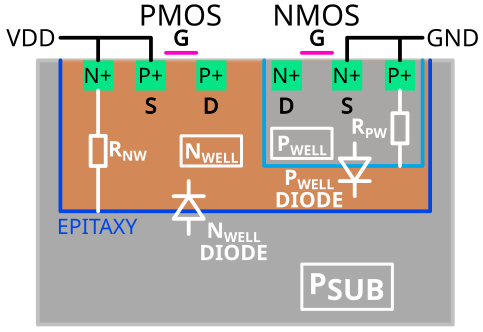
\includegraphics[width=7.8cm]{3_modeling/figures/TRIPLE.pdf}
        \caption{Triple-Well}
        \label{subfig:tripleIvx}
    \end{subfigure}
    \caption{Dual-well and triple-well inverter silicon sectional view.}
    \label{fig:dualTripleIvx}
\end{figure}
On one hand, when performing EMFI (usually on the front side of the IC), air is the physical support to convey energy through electromagnetic waves.
It is achieved by coupling the loop wire probe to the power delivery network loops.
On the other hand, when working with BBI, the context is different.
Indeed, the energy is conveyed through electrical charges through the silicon substrate.
Therefore, the carriers have to go through the metallic probe and the whole substrate to reach the logic gates and the power delivery network in order to disturb the IC operation.
Thus, the substrate type and design could have a significant impact on BBI efficiency.
As a result, we explored and studied BBI in two specific scenarios depending on the substrate types: dual-well and triple-well.
Fig. \ref{fig:dualTripleIvx} shows the sectional views of two inverters manufactured in a dual-well and a triple-well substrate respectively.
These simple schematics are helpful in understanding the reasoning behind the design of the electrical models.

Fig. \ref{subfig:dualIvx} depicts the cross-sectional view of a dual-well CMOS inverter.
The P-doped silicon substrate is colored in gray, with $RC_{GND}$ being the access resistance from the epitaxy layer to the NMOS bulk.
This physical environment is the conducting support of electrical charges which flow up to the NMOS transistor.
The orange region is the N-doped silicon well, located inside the P-substrate to manufacture the PMOS transistors.
$RC_{VDD}$ is the access resistance from the epitaxy to the PMOS bulk inside the $N_{WELL}$.
In addition to the P-substrate, the N-well is the last environment electrical charges have to go through before reaching the PMOS transistor.

Fig. \ref{subfig:tripleIvx} shows the cross-sectional view of a triple-well CMOS inverter.
As before, gray areas represent P-doped silicon, and orange areas N-doped silicon.
$R_{NW}$ is the $N_{WELL}$ access resistance from the epitaxy to the PMOS bulk, and $R_{PW}$ is the $P_{WELL}$ access resistance from the $N_{WELL} - P_{WELL}$ junction to the NMOS bulk.
In this case, two silicon junctions are present, represented by two independent diodes.
In order to reach the PMOS transistors, charges have to go through the exact same environments as before.
However, concerning NMOS transistors, they have to pass through two silicon junctions instead of none.
As discussed in Chapter \ref{chap:5faultModel}, this has a significant impact on BBI induced effects.
However, these schematics are incomplete and do not allow simulating ICs behaviors under BBI.

Therefore, as it has been done in \cite{mathieuEMFI}, ICs are spatially split in elementary sections called standard-cells segments (SCS).
However, in addition to the improvement of the dual-well proposed model proposed in \cite{mathieuEMFI}, we also introduce a triple-well model in order to fully appreciate the behavioral differences of BBI applied to both substrate types.

%\begin{figure}[ht]
    \centering
    \includegraphics[width=0.65\textwidth]{3_modeling/figures/substrateSubdivision_6.pdf}
    \caption{Substrate subdivision improvement over M. Dumont model for \emfi \cite{mathieuEMFI}. The backside is the accessible substrate, and the epitaxy is the highest substrate level, a.k.a. the silicon junction between the P-substrate and the N-well.}
    \label{fig:surfaceSubDivid}
\end{figure}
%\begin{figure}[ht]
    \centering
    %\scriptsize
    % \setstretch{0.9}
    \begin{subfigure}{0.45\textwidth}
        % \def\svgwidth{9.0cm}
        \includegraphics[width=\textwidth]{3_modeling/figures/dualWell_no_5e.pdf}
        \caption{Dual-Well}
        \label{subfig:dualScs}
    \end{subfigure}
    \hfill
    \begin{subfigure}{0.45\textwidth}
        % \def\svgwidth{9.0cm}
        \includegraphics[width=\textwidth]{3_modeling/figures/tripleWell_no_5e.pdf}
        \caption{Triple-Well}
        \label{subfig:tripleScs}
    \end{subfigure}
    \caption{Three-dimensional Dual-Well and Triple-Well IC comprehensive standard-cell electrical schematic.}
    \label{fig:dualTripleScs}
\end{figure}
The main improvement over the dual-well model proposed in \cite{mathieuEMFI} concerns the substrate resistive network, as shown in Fig. \ref{fig:surfaceSubDivid}.
In \cite{mathieuEMFI}, the substrate network is coarse and only consists of six electrical resistances for each SCS.
It means that they represent the entire SCS substrate thickness, width, and height (on the left in Fig \ref{fig:surfaceSubDivid}).
Even though it is sufficient to appreciate the injection method effects while studying EMFI, mainly because the substrate is almost transparent when it comes to electromagnetic waves, but also because EMFI is mostly performed at the IC front side, it is not precise enough to model the spreading of he voltage pulse from the IC backside to the transistors.

To that end, we decided to split as much as possible these resistors, as shown in Fig. \ref{fig:surfaceSubDivid}, to provide a precise enough substrate sub-model while keeping realistic computational workload.
For the final models, it was decided to use an editable elementary thickness of $10 \; \mu m$, and fixed width and depth of $5 \; \mu m$ for each elementary six-resistors substrate models, according to the footprint of an SCS on the XY plane ($5 \; \mu m \; \times \; (6 \; \mu m \; \times \; 5 \; \mu m)$), resulting in a $30 \; \mu m$ wide and $5 \; \mu m$ deep SCS.
One can remark that in Fig \ref{fig:dualTripleScs}, no number is given concerning the substrate thickness, as similar to LFI, it is an important parameter which does not have a fixed value.
Indeed, an attacker may want to thin the substrate or not before performing BBI.

Furthermore, as shown in Fig. \ref{fig:dualTripleScs}, both SCS models contain various electrical components describing the IC structure, roughly composed of:
\begin{itemize}
    \item Its substrate
    \item Its silicon junction(s)
    \item Its logic gates
    \item Its power supply rails
\end{itemize}
These two models, while being close to each other, allow, thanks to their subtle differences, to properly consider the different behaviors each substrate type exhibits.
In the next section, dual-well SCS model and triple-well SCS model are consecutively considered and analyzed.

\subsection{Standard-cell segment models \ddc}
\label{subSect:dualTripleWellScs}
Historically, IC substrate was manufactured using an exclusive dual-well structure.
However, nowadays, it is common to find on relatively modern ICs a mix of dual-well and triple-well structures on a monolithic die.
Triple-well substrate structures bring significant advantages over dual-well substrates.
In digital ICs, it is mainly used to body bias transistors to optimize their performance under power constraints.
When used in analog or mixed designs, it gives two main advantages: substrate cross-talk and noise reduction, in addition to power supply decoupling thanks to the additional P-N junction capacitance \cite{tripleWellDecoupling}.
This is why we decided to cover dual-well and triple-well structures in our models.

Fig. \ref{subfig:dualScs} depicts an SCS dual-well model.
Each significant section of the SCS is gray-framed and numbered:
\begin{itemize}
    \item The section \ovalbox{1} represents the substrate environment: resistive and isotropic.
    \item The section \ovalbox{2} is the $P-N$ silicon junction between the P-substrate and the N-well, represented by a diode and its junction capacitance, in addition to an access resistance $RC-VDD$, being the N-well electrical resistance.
    \item The section \ovalbox{3} is the substrate access resistance.
    \item The sections \ovalbox{4P} and \ovalbox{4N} contain the average non-logical model of a hundred of logic gates.
    \item The sections \ovalbox{5} and \ovalbox{5'} are the two levels of the power delivery network, which are low resistive metals.
    \item The section \ovalbox{6} is the decoupling between both $GND$ and $V_{DD}$ power networks.
\end{itemize}

Fig. \ref{subfig:tripleScs} depicts the SCS triple-well model as follows:
\begin{itemize}
    \item The section \ovalbox{2} is the $P-N$ silicon junction between the P-substrate and the N-well, represented by a diode and its junction capacitance, in addition to an access resistance $R_{NW}$, being the N-well electrical resistance.
    \item The section \ovalbox{3} is the $N-P$ silicon junction between the N-well and the P-well, represented once again by a diode and its junction capacitance, in addition to an access resistance $R_{PW}$, being the P-well electrical resistance.
    \item The sections \ovalbox{1}, \ovalbox{4P}, \ovalbox{4N}, \ovalbox{5'} and \ovalbox{6} being the same as before.
\end{itemize}

\begin{figure}[H]
    \centering
    \includegraphics[width=0.5\textwidth]{3_modeling/figures/algoFigure5.png}
    \caption{Elementary substrate 3D netlist}
    \label{fig:algo}
\end{figure}
\algdef{SE}% flags used internally to indicate we're defining a new block statement
[CLASS]% new block type, not to be confused with loops or if-statements
{Class}% "Class{name}" will indicate the start of the struct declaration
{EndClass}% "EndClass" ends the block indent
[1]% There is one argument, which is the name of the class
{\textbf{class} \textsc{#1}}% typesetting of the start of a struct
{\textbf{end class}}% typesetting the end of the struct

\algdef{SE}% flags used internally to indicate we're defining a new block statement
[METHOD]% new block type, not to be confused with loops or if-statements
{Method}% "Method{name}" will indicate the start of the struct declaration
{EndMethod}% "EndMethod" ends the block indent
[2]% There is one argument, which is the name of the data structure
{\textbf{method} \textsc{#1}}% typesetting of the start of a struct
{\textbf{end method}}% typesetting the end of the struct

\begin{figure}[H]
    \begin{Verbatim}[frame=single]
        .subckt elementary_bloc D F L R Re U
        R1 U N001 RH
        R2 N001 D RH
        R3 Re N001 RL
        R4 N001 F RL
        R5 N001 L RL
        R6 R N001 RL
        .ends elementary_bloc
    \end{Verbatim}
    \caption{Elementary substrate SPICE netlist}
    \label{fig:subSpiceNetlist}
\end{figure}

\begin{figure}[H]
    \begin{Verbatim}[frame=single]
    .subckt elementary_blocx6 D1 D2 D3 D4 D5 D6
    +F1 F2 F3 F4 F5 F6 L R RE1 RE2 RE3 RE4 RE5 RE6
    +U1 U2 U3 U4 U5 U6 VSUBCintC
    XX1 D1 F1 L VSUBCintL2 RE1 U1 elementary_bloc
    XX2 D2 F2 VSUBCintL2 VSUBCintL1 RE2 U2 elementary_bloc
    XX3 D3 F3 VSUBCintL1 VSUBCintC RE3 U3 elementary_bloc
    XX4 D4 F4 VSUBCintC VSUBCintR1 RE4 U4 elementary_bloc
    XX5 D5 F5 VSUBCintR1 VSUBCintR2 RE5 U5 elementary_bloc
    XX6 D6 F6 VSUBCintR2 R RE6 U6 elementary_bloc
    .ends elementary_blocx6
    \end{Verbatim}
    \caption{SCS substrate layer SPICE netlist}
    \label{fig:subSpiceSCS}
\end{figure}

%\begin{figure}[!h]
%    \begin{Verbatim}[frame=single]
%    R1 vic vlt Rmup/4
%    R2 vlt vi1c Rmup/4
%    RM1 vddc vlt RM1/4
%    Ra_TL1 vddc N001 Ra
%    Cdecp_L1 N001 gndc Cdecp
%    Cdecp_R1 vddc N002 Cdecp
%    Ra_BR1 N002 gndc Ra
%    RM2 gndc glb RM1/4
%    R3 gic glb Rmup/4
%    R4 glb gi1c Rmup/4
%    RM3 grb gndc RM1/4
%    RM4 vrt vddc RM1/4
%    R5 gic1 grb Rmup/4
%    R6 grb gi1c1 Rmup/4
%    R7 vrt vi1c1 Rmup/4
%    R8 vic1 vrt Rmup/4
%    vepi_curr vepi vepi_meas dc=0
%    Rn1 gndc ncgnmos RN
%    Rp1 vddc ncgpmos RP
%    cgp_n1 ncgnmos vgp cgp
%    cgn_n1 ncgnmos vepi_meas cgn
%    cgn_p1 ncgpmos vepi_meas cgn
%    cgp_p1 ncgpmos vgp cgp
%    RCVDD vddc vgp RcontactDW
%    CNWPS vgp vepi_meas cnw
%    RCGND gndc vepi_meas RcontactDW
%    xDNWPS vepi_meas vgp dnwps AREA=31.43u PJ=70u
%    \end{Verbatim}
%    \caption{Dual-well standard-cell upper section netlist}
%    \label{fig:SCSdualUp}
%\end{figure}
%
%\begin{figure}[!h]
%    \begin{Verbatim}[frame=single]
%    R1 vic vlt Rmup/4
%    R2 vlt vi1c Rmup/4
%    RM1 vddc vlt RM1/4
%    Ra_TL1 vddc N001 Ra
%    Cdecp_L1 N001 gndc Cdecp
%    Cdecp_R1 vddc N002 Cdecp
%    Ra_BR1 N002 gndc Ra
%    RM2 gndc glb RM1/4
%    R3 gic glb Rmup/4
%    R4 glb gi1c Rmup/4
%    RM3 grb gndc RM1/4
%    RM4 vrt vddc RM1/4
%    R5 gic1 grb Rmup/4
%    R6 grb gi1c1 Rmup/4
%    R7 vrt vi1c1 Rmup/4
%    R8 vic1 vrt Rmup/4
%    vepi_curr vepi vepi_meas dc=0
%    Rn1 gndc RNCN RN
%    Rp1 vddc RPCP RP
%    cgp_n1 VPsNw RNCN cgp
%    cgn_n1 RNCN VNwPw cgn
%    cgn_p1 RPCP VNwPw cgn
%    cgp_p1 VPsNw RPCP cgp
%    RNW1 VPsNw vddc RcontactTW
%    cnw1 VPsNw vepi_meas cnw
%    RPW1 gndc VNwPw RcontactTW
%    xdpsnw1 vepi_meas VPsNw dnwps AREA=15.72u PJ=40u
%    xdnwpw1 VNwPw VPsNw dnwps AREA=31.43u PJ=70u
%    cnw2 VNwPw VPsNw cnw
%    cnw3 VPsNw vepi_meas cnw
%    xdpsnw2 vepi_meas VPsNw dnwps AREA=15.72u PJ=40u
%    \end{Verbatim}
%    \caption{Dual-well standard-cell upper section netlist}
%    \label{fig:SCStripleUp}
%\end{figure}

%\begin{algorithm}[H]
%    \caption[ic algo func]{Generation algorithm classes and function}
%    \label{alg:genFuncClass}
%    \begin{algorithmic}
%        \Class{NetlistTextFile} \Comment{Object defining the netlist to be generated}
%        \State \textbf{text}: String content of the class
%        \State $write(value : String)$: Write characters into the parent class "\textbf{text}" attribute
%        \EndClass\\
%
%        \Class{DualWellSCS} \Comment{Dual-well standard-cell netlist}
%        \State \textbf{text}: String content of the class
%        \State $read()$: Read characters into the parent class "\textbf{text}" attribute
%        \EndClass\\
%
%        \Class{TripleWellSCS} \Comment{Triple-well standard-cell netlist}
%        \State \textbf{text}: String content of the class
%        \State $read()$: Read characters into the parent class "\textbf{text}" attribute
%        \EndClass\\
%
%        \Function{createNets}{X : float, Y : float, NET : String}
%        \State \Comment{Create nets to connect SCS together}
%        \State $NetArray \gets ???$
%        \State \Return NetArray
%        \EndFunction\\
%
%        \Function{writeInMainNetlist}{value : String}
%        \State \Comment{Write generated results into main netlist}
%        \State NetlistTextFile.write(value)
%        \EndFunction\\
%
%        \Function{subRHcalc}{ESUB : int, RH : float, RL : float}
%        \State \Comment{Calculate elementary substrate resistors}
%        \State $RH \gets RH \times (ESUB \div 10)$
%        \State $RL \gets RL \times (ESUB \div 10)$
%        \State \Return RH, RL
%        \EndFunction\\
%
%        \Function{SCSelemGen}{SUBTYPE} \Comment{Generate Standard Cell Segment Model}
%        \If{$SUBTYPE = DualWell$}
%        \State $SCSNetlistDW = DualWellSCS$
%        \State $SCSNetlistTW = None$
%        \ElsIf{$SUBTYPE = TripleWell$}
%        \State $SCSNetlistDW = None$
%        \State $SCSNetlistTW = TriplelWellSCS$
%        \ElsIf{$SUBTYPE = Mixed$}
%        \State $SCSNetlistDW = DualWellSCS$
%        \State $SCSNetlistTW = TriplelWellSCS$
%        \EndIf
%        \State $SCSNetlistArray \gets {SCSNetlistDW, SCSNetlistTW}$
%        \State \Return SCSNetlistArray
%        \EndFunction\\
%    \end{algorithmic}
%\end{algorithm}

\begin{algorithm}[H]
\caption[ic algo]{Integrated circuit SPICE netlist generation algorithm.}
\label{alg:icGen}
\begin{algorithmic}
    \Require SUBTYPE \Comment{IC substrate type: Dual-well, Triple-well, Mixed}
    \Require TSUB \Comment{IC substrate thickness}
    \Require ESUB \Comment{Elementary substrate block thickness}
    \Require VPUU \Comment{Voltage pulse amplitude}
    \Require PW \Comment{Voltage pulse width}
    \Require TFR \Comment{Voltage pulse rise and fall times}
    \Require SIMTIME \Comment{Simulation duration}
    \Require SIMSTEP \Comment{Simulation time step}
    \Require TEX \Comment{Desired X size (µm)}
    \Require TEY \Comment{Desired Y size (µm)}
    \State $RH \gets 2000$ \Comment{Elementary substrate up-down/front-rear resistor value}
    \State $RL \gets 500$ \Comment{Elementary substrate left-right resistor value}
    \State $WSEG \gets 30$
    \State $HSEG \gets 5$
    \State $W6SEG \gets 30 \div 6$
    \State $nC \gets TEX \div WSEG$ \Comment{Number of column}
    \State $nL \gets TEY \div HSEG$ \Comment{Number of lines}
    \State $nH \gets TSUB \div ESUB$ \Comment{Number of substrate layers}
    \Ensure nC, nL and nH are integers
%    \State $RH, RL \gets \Call{subRHcalc}{ESUB, RH, RL}$
    \State $RH \gets RH \times (ESUB \div 10)$ \Comment{Adjust RH value according to user defined variable}
    \State $RL \gets RL \times (ESUB \div 10)$ \Comment{Adjust RL value according to user defined variable}
    \ForAll{cY in [0; nL[}
        \ForAll{cX in [0; nH[}
            \State $\overrightarrow{X} \gets
            \left[\begin{array}{r}
                        cX \times WSEG\\
                        cX \times WSEG + 1 \times (W6SEG \div 2)\\
                        cX \times WSEG + 3 \times (W6SEG \div 2)\\
                        cX \times WSEG + 5 \times (W6SEG \div 2)\\
                        cX \times WSEG + 7 \times (W6SEG \div 2)\\
                        cX \times WSEG + 9 \times (W6SEG \div 2)\\
                        cX \times WSEG + 11 \times (W6SEG \div 2)\\
                        cX \times WSEG + 12 \times (W6SEG \div 2)\\
                \end{array}\right]$
            $;\overrightarrow{Y} \gets
            \left[\begin{array}{r}
                        cY \times HSEG\\
                        (cY + \frac{1}{2}) \times HSEG\\
                        (cY + 1) \times HSEG\\
                \end{array}\right]$
            \State $;\overrightarrow{P} \gets
            \left[\begin{array}{r}
                cY \times HSEG\\
                (cY + \frac{1}{2}) \times HSEG\\
                (cY + 1) \times HSEG\\
            \end{array}\right]$
        \EndFor
    \EndFor
    \State \textcolor{orange}{TO FINISH.}
\end{algorithmic}
\end{algorithm}

Each area of the elementary SCS models were automatically generated using  a custom algorithm, shown in Alg. \ref{alg:icGen}.
It was mainly designed in order to reduce as much as possible any human intervention to limit difficult to debug errors and inconsistencies.
Furthermore, it provides a degree of flexibility due to the ease of user modifications directly into the generation algorithm parameters, as opposed to netlist editing, thereby reducing errors further.
These models only represent a section of an integrated circuit. For effective use and verification, it is necessary to replicate and interconnect these models spatially as much as possible.
This was accomplished by utilizing customized Python scripts coupled with procedural generation.
The IC generation algorithm enables the modification of multiple settings to produce the desired outcomes, albeit with certain inherent structural limitations.
Two of the main limitations are the fixed width and depth of the elementary SCS models, and the fixed number of metal levels in the power delivery network.
On the contrary, the following is a non-exhaustive list of user-modifiable settings:
\begin{itemize}
	\item Global IC size.
	\item Probe position.
	\item IC global substrate thickness.
	\item IC elementary substrate thickness.
	\item Substrate type (dual-well, triple-well, or mixed).
	\item Voltage pulse amplitude.
	\item Voltage pulse width.
	\item Voltage pulse rise and fall times.
	\item Simulation time and step.
\end{itemize}
Eventually, the generator script incorporates a visual inspection tool in order to quickly verify the correctness of the generated netlist.
Alg. \ref{alg:icGen} shows the IC generation algorithm main function, which is to create the coordinates for every net in the netlist.
%Alg. \ref{alg:icGen} presents the IC generation algorithm, alongside Fig. \ref{fig:algo}.
